\documentclass[11pt]{article}
\usepackage{setspace}
\usepackage{graphicx} % Required for inserting images
\usepackage{hyperref}
\usepackage{ragged2e}
\usepackage{longtable}
\usepackage{array}
\usepackage{booktabs}
\usepackage{fontspec}
\usepackage{moresize}
\usepackage[table]{xcolor}
\usepackage[left=2.54cm, right=2.54cm, top=2.54cm, bottom=2.54cm]{geometry}
%\showframe
\newcolumntype{L}[1]{>{\RaggedRight\centering\hyphenchar\font=`\-\arraybackslash}p{#1}}
\hypersetup{
    colorlinks,
    linkcolor = {red!50!black},
    citecolor = {blue!50!black},
    urlcolor = {blue!80!black}
}
\setstretch{1.5}
\usepackage[
backend=biber,
style=numeric,
sorting=ynt
]{biblatex}
\addbibresource{project_references_latex.bib}
\bibliography{references}
\setmainfont{Arial}
\newfontfamily\seriffont{Times New Roman}
\begin{document}
\title{Machine Learning Prediction of Intensive Care Length of Stay for Lung Cancer Patients}
\author{Louis Bolduc}
\date{September 2024}

\maketitle
\tableofcontents
\pagebreak

\begin{abstract}
    
\end{abstract}

\renewcommand{\abstractname}{Acknowledgements}
\begin{abstract}
 
\end{abstract}

\section{Introduction}

\subsection{Aims and Objectives}
The main aim of this project is to build accurate and efficient machine learning models using data from the MIMIC dataset to enhance the prediction of the length of stay in the Intensive Care Unit, ICU, for lung cancer patients. The ideal result would be for this to benefit personalised healthcare and resource management in oncology.

The main aims and objectives are the following:
\begin{itemize}
    \item Aim 1 - Extract the data from the MIMIC dataset to form a final dataset ready to be used to develop predictive models.
	\begin{itemize}
	\item Objective 1 - Determine the variables for selection 
	\item Objective 2 - Setup the MIMIC database on PostgresSQL
	\item Objective 3 - Extract the data
	\item Objective 4 - Clean the data
	\end{itemize}
    \item Aim 2 - Train various predictive models.
	\begin{itemize}
	\item Objective 1 - Cross-validate 
	\item Objective 2 - Impute the missing data
	\item Objective 3 - Linear regression model
	\item Objective 4 - Penalistation models
	\item Objective 5 - Random forest
	\end{itemize}
    \item Aim 3 - Evaluate the models assessing the effectiveness of each. 
	\begin{itemize}
	\item Objective 1 - Calculate performance metrics
	\item Objective 2 - Compare models
	\item Objective 3 - Compare findings with other studies
	\end{itemize}
\end{itemize}

\subsection{Background to Lung Cancer and ICU Treatment}
Cancer is a disease that involves the uncontrollable multiplication of malignant cells, in some cases forming tumours in organs or tissues. In the US, and many other countries around the world, cancer has become the leading cause of death, and in the US specifically it has been reported that around 1 in 3 people will be diagnosed with any cancer and 1 in 6 of cancer mortality in their lifetimes. This statistic indicates that the volume of patients requiring ICU treatment will be significantly large and therefore the optimisation of length of stay analysis is key to resource management and patient care planning. Lung cancer in particular describes the cancerous cell growth in the lungs and is regarded as a serious health issue for both the patient and healthcare systems worldwide.

According to the official WHO global cancer observatory, lung cancer is the cancer with the highest percentage of mortality and one of the most prevelant. To link this to the statistic previously mentioned, lung cancer will develop in approximately 1 in 17 and be the cause of death in 1 in 28 of Americans. This prevelance and mortality differs when broken down by sex and lung cancer is not the most prevelant or most deadly cancer for women, breast cancer is, however when addressing the whole population lung cancer is the cancer that poses the biggest threat. Focusing on the one cancer that is singled out as the most threatening allows for a more concentrated study that should in theory generate more useful results. 

As of Joohyn Park., et al's 2019 report, the mean annual health care expenditure for a lung cancer patient in the US is \$35,141. This was significantly higher than the 4 most common cancer types that were included and approximately 8-9 times as high for a cancer free patient, \$4484. These numbers point towards the extent of how significant the burden of lung cancer is on the US healthcare system. They also report that lung cancer tends to be diagnosed at more advanced stages so the survival duration is short with a 5-year survival rate estimated at 18.6\%. With a higher number of cases diagnosed at advanced stages, intensive care units are expected to be required to administer treatment to patients.

%Malignant cancer cells in the body often escape detection, limiting the ability of the immune system to prevent their spread and mitigate the resulting damage. Immunotherapy is a treatment that boosts the immune response and prevents cancer cells from suppressing it, enabling the immune system to detect and destroy cells more effectively. For early stage lung cancer, stages I-III, immunotherapy is still not considered the most effective form of treatment in most cases; however, a significant proportion of patients in the latter stages of the disease will receive some form of this treatment.

%\subsection{Length of Stay Prediction}
The length of stay in an ICU ward is an important piece of information for clinicians to know and if it can be predicted accurately the efficiency of the intensive care process would improve and so would the quality of care provided. At the time of writing, although some machine learning predictions of ICU length of stay are being researched and perhaps trialled in a limited amount of hospitals, the majority of healthcare systems go by clinical judgement alone. One of the main reasons behind this stems from the lack of understanding regarding how to pair the machine learning assistance to the clinician's expertise in a way that optimises the blend of predictive knowledge that both provide\cite{MachineLearningOpportunities}. The lack of use of these methods in practice provides a rationale for conducting this type of study.

\subsection{Machine Learning}

\subsubsection{What is Machine Learning?}

The advancement of computational power and access to large amounts of data has created an opening for the application of statistical techniques to develop machine learning algorithms to produce potentially quite accurate and useful results. Machine learning works similarly to the human brain in that it takes in input information and uses it to build a form of understanding of abstract concepts. Computers will attempt to learn from their input data to identify patterns for use in making predictions or in producing analyses.

There are some things to consider when creating a machine learning model. A model that is trained on data from a specific portion of a population, for example a model that is trained on data from people of a specific country, creates selection bias which renders the model less useful for the rest of the population. So one way to combat this would be to retrain the model on data specific to the population it is intended to be used for. There is also the case of overfitting and underfitting. An underfitted model fails to identify the patterns in the data which may come down to too few variables. An overfitted model is practically the opposite, the model fits too well on the data given therefore performing less well on new data. Adressing these challenges is key to creating and deploying a significantly useful model. 

\subsubsection{Possible Benefits}

At current clinicians do not use machine learning techniques to predict length of stay for lung cancer ICU patients. Their predictions or estimates almost primarily come down clinical judgement. Therefore estimates may be more accurate depending on the experience of the clinician. It is also not an immediate priority of the clinician, they may have the most granular knowledge but they are more focused on administering the best possible treatment to their patients. Therefore a clinically significant machine learning prediction model could help as an aide for hospital staff to make good approximations of the length of stay for an individual patient.

Due to factors such as an aging population, medical advancements and staffing shortages, ICUs have now a greater utilisation for severe medical complications such as lung cancer. This raises a few challenges that being able to produce a reliable estimate of a patient's length of stay would be useful for.

First of all, it is imperative for hospital staff to have an understanding of bed availability so that they can manage the influx of new patients effectively. Knowing which beds may shortly become available helps ward managers plan ahead for incoming patients and provides an estimate of how many beds an ICU ward may need. 

The knowledge of how long a patient will stay on the ward is a useful bit of information for managing costs. Since longer stays mean higher costs, length of stay predictions can be used to estimate how much a hospital needs to be spending on the ICU ward which distinguishes how much of a hospitals overal budget goes toward the ICU.

\subsection{The MIMIC Database}
MIMIC is a large relational database that consists of deidentified data collated from thousands of admissions to the intensive care unit of the Beth Israel Deaconess Medical Centre in Boston, Massachusetts. The acronym MIMIC has stood for "Multiparameter Intelligent Monitoring in Intensive Care" and more recently "Medical Information Mart for Intensive Care". Some key features of this database are that it is the only freely accessible critical care database of its kind and contains detailed information on patients spanning more than a decade. The most recent version of the MIMIC database is MIMIC-IV which includes, most importantly, data all the way up to the year 2019 as opposed to 2012 for MIMIC-III. Using the updated version should allow for greater relevance and accuracy of the prediction model. The value of MIMIC in this study lies in the comprehensive real-world data it contains, which enables the model to train more accurately compared to synthetic data, allowing it to fit better to unseen data.

Data can be accessed after completing a short ethics course set up by the CITI programme website.[citeMIMICethics]

\subsection{Literature Review}

This literature review aimed to find relevant peer-reviewed publications to compare with the findings of this study, and to inform on the existing research and the reported results found in this area. The criteria for the initial search were: population of adults over 18, lung cancer ICU studies, length of stay prediction with machine learning, a result of the predictive performance should be stated.  A search with these parameters in PubMed found 5 results of which none were relevant. So the search parameters needed to be broadened. The age restriction was dropped and so was the specifity of lung cancer, as in any ICU LOS machine learning prediction study was considered. This search in PubMed produced 697 results of which 13 fit this criteria.

Additionally, 1 publication was found outside of PubMed that fit all of the initial criteria. 

{\seriffont
{\small
\renewcommand{\arraystretch}{1}
\centering
\begin{center}
\setlength{\arrayrulewidth}{0.7mm}
\begin{longtable}{ |L{2cm} | L{1cm} | L{4cm} | %L{5cm} |
 L{6cm} | L{2cm} |} 
    \hline
    \textbf{Author} & \textbf{Year} & \textbf{Prediction Model} & \textbf{Best Model} %& \textbf{Predictor Variables}
 & \textbf{Data Source} \\ 
    \noalign{\global\setlength{\arrayrulewidth}{0.7mm}}
    \hline
    \endfirsthead

\hline
\textbf{Author} & \textbf{Year} & \textbf{Prediction Model} & \textbf{Best Model} %& \textbf{Predictor Variables}
 & \textbf{Data Source} \\
\hline
\endhead
  Ilona W.M.Verburg., et al  & 2014 & OLS regression, OLS regression truncated at 30 days, OLS regression log, GLM Gaussian, GLM poisson, GLM negative binomial, GLM Gamma, Cox PH regression & OLS regression truncated at 30 days: R$^2$ - 0.208 (0.2001 to 0.215), RMSPE - 5.150 (5.061 to 5.239), MAPE - 3.099 (3.053 to 3.144), BIAS - 0.015 (-0.044 to 0.074) &%  Number of ICU admissions, ICU LOS in days, Age in year, Sex, Admission type, APACHE IV APS, Ventilation within first 24hrs of ICU admission, One or more chronic diseases, One or more diagnoses at admission, Confirmed infection, Use of vasoactive drugs, Lowest GCS first 24hrs, Non-operative APACHE IV diagnosis category, Post-operative APACHE IV diagnosis category &
 NICE\\ 
    \noalign{\global\setlength{\arrayrulewidth}{0.05mm}}
    \hline
    \noalign{\global\setlength{\arrayrulewidth}{0.7mm}}
  Qiuying Chen, et al  & 2021 & Naive Bayes, Linear Regression, Decision Tree, Random Forest, Gradient Boosting Decision Tree & Random Forest: AUC - 0.991 (0.978 to 1.000) and 0.837 (0.766 to 0.908) in the training and validation datasets respectively &%  Preoperative (Demographics, Clinical manifestations, medication history, previous history, vital signs, labratory findings and auxilary examinations), Intraoperative (Surgical types, Surgical times, Surgical technique and Intraoperative observation) &
 Guangdong Provincial Cardiovascular Institute \\ 
    \noalign{\global\setlength{\arrayrulewidth}{0.05mm}}
    \hline
    \noalign{\global\setlength{\arrayrulewidth}{0.7mm}}
 Khalid Alghatani., et al  & 2021 & Linear Regression, Linear Discriminant Analysis, Random Forest, k-Nearest Neighbour, Support Vector Machine, XGBoost, Multivariate Linear Regression, Support Vector Regression & Random Forest &% Heart rate, Arterial systolic blood pressure, Respiratory rate, Body temperature, Arterial diastolic blood pressure, Peripheral oxygen saturation, Blood glucose, Age, Sex, Height, Weight & 
MIMIC-III \\ 
    \noalign{\global\setlength{\arrayrulewidth}{0.05mm}}
    \hline
    \noalign{\global\setlength{\arrayrulewidth}{0.7mm}}
 Longxiang Su., et al  & 2021 & Logistic Regression, Random Forest, XGBoost & Random Forest: AUC - 0.76 & %Age, Perfusion index, P(v-a)CO$_2$/C(a-v)O$_2$pCO$_2$, Noradrenaline dosage, Adrenaline dosage, Invasive blood pressure, Central venous pressure, P(v-a)CO$_2$(mmHg), sO$_2$, Lactic acid, Invasive systolic blood pressure, Invasive diastolic blood pressure, Oxygenation index, White blood cell, Platelet count, Total bilirubin, GCS score, Creatine, Oxygen concentration, SpO$_2$, pO$_2$, Heart rate, Body temperature, Respiratory rate, SOFA score  & 
ICU unit of Peking Union Medical College Hospital \\ 
    \noalign{\global\setlength{\arrayrulewidth}{0.05mm}}
    \hline
    \noalign{\global\setlength{\arrayrulewidth}{0.7mm}}
 Andrea Stieger., et al  & 2025 & Logistic Regression, Random Forest, Stacked Learner, Gradient Boosting Machine, Neural Networks & Stacked Learner: AUROC - 0.94, AUPRC - 0.62 &% Preoperative (Haemoglobin, Platelet count, Prothrombin time, Activated partial thromboplastin time, Sodium, Potassium, Glucose, Albumin, Asparate transterase, Alanine transferase, Blood urea nitrogen, Creatine), Intraoperative (Glucose, bicarbonate, Haematocrit, Ionised calcium, Potassium, Lactate, Sodium, Partial pressure of CO$_2$, pH, Partial pressure of O$_2$, Arterial oxygen saturation &
 Seoul National University Hospital\\ 
    \noalign{\global\setlength{\arrayrulewidth}{0.05mm}}
    \hline
    \noalign{\global\setlength{\arrayrulewidth}{0.7mm}}
 Louise Y.Sun., et al  & 2020 & Logistic Regression & Short stay: c-statistic (0.78/ 0.71, derivation/validation), Long stay: c-statistic (0.85/0.78, derivation/validation) This essientially concludes the idea that the logistic regression model may help practictioners &% Age, Body mass index, NYHA classification, LVEF, GFR, Operative characteristics, Type of surgery &
 University of Ottawa Heart Institute\\ 
    \noalign{\global\setlength{\arrayrulewidth}{0.05mm}}
    \hline
    \noalign{\global\setlength{\arrayrulewidth}{0.7mm}}
 Kan Wang., et al  & 2022 & Linear Regression, Naive Bayes, Random Forest, Support Vector Machine, XGBoost & XGBoost: AUC - 0.88 &% Recipient age, Donor age, Donor gender, BMI ratio, Recipient blood type, Blood type match, NYHA, Cardiovascular surgery, Smoking, Alcohol, K$^+$, ALT, AST, Cr, INR, BNP, LDL, Renal complication, Hepatic complication, Hypertension, Diabetes, Extracorporeal circulation time, Aortic cross clamp time, Surgery time, Chest re-exploration, IABP, ECMO, CRRT &
 Wuhan Union Hospital\\ 
    \noalign{\global\setlength{\arrayrulewidth}{0.05mm}}
    \hline
    \noalign{\global\setlength{\arrayrulewidth}{0.7mm}}
 Pepler PT., et al  & 2012 & Poisson Log-linear, Regression Model & Logistic Regression - AUC 0.8507 &% Apgar at 1 min, Apgar at 5 min, Temperature, Birth head circumference, Birth weight, Gestational age, Region, Maternal ethnicity, Delivery mode, Gender &
 Vermont Oxford Network\\ 
    \noalign{\global\setlength{\arrayrulewidth}{0.05mm}}
    \hline
    \noalign{\global\setlength{\arrayrulewidth}{0.7mm}}
 Yucai Hong., et al  & 2020 & Multivariate Regression Model & Multivariate Regression Model: AUC - 0.848 &% see paper and add in & 
Tertiary Care Hospital in Yueqing City, Zheijiang Province\\ 
    \noalign{\global\setlength{\arrayrulewidth}{0.05mm}}
    \hline
    \noalign{\global\setlength{\arrayrulewidth}{0.7mm}}
 Geert Meyfroidt., et al  & 2011 & Logistic Regression, Decision Trees, Random Forest, Support Vector Machines, Gaussian Forest & Gaussian Processes: RMSE - 0.408, AUC - 0.758 &% Not well defined in the paper &
 MetaVision PDMS Database\\ 
    \noalign{\global\setlength{\arrayrulewidth}{0.05mm}}
    \hline
    \noalign{\global\setlength{\arrayrulewidth}{0.7mm}}
 Waqar Aziz., et al  & 2024 & Random Forest, Gradient Boosting & Gradient Boosting: AUC - 0.7243 &% Triage Acuity, Disposition admitted, Elixhauser Comorbidity Index (ECI), Arrival transport unknown, Arrival transport ambulance chief compliant abdominal pain, Age, Disposition transfer, Chief compliant chest pain, Disposition HOME &
 MIMIC-IV-ED\\ 
    \noalign{\global\setlength{\arrayrulewidth}{0.05mm}}
    \hline
 \noalign{\global\setlength{\arrayrulewidth}{0.7mm}}
 Belal Alsingwali., et al  & 2022 & Random Forest, XGBoost, Logistic Regression & Random Forest: k-fold = 10 mean accuracy - 87.4\% &% Triage Acuity, Disposition admitted, Elixhauser Comorbidity Index (ECI), Arrival transport unknown, Arrival transport ambulance chief compliant abdominal pain, Age, Disposition transfer, Chief compliant chest pain, Disposition HOME &
 MIMIC-III\\ 
    \noalign{\global\setlength{\arrayrulewidth}{0.05mm}}
    \hline
    \noalign{\global\setlength{\arrayrulewidth}{0.7mm}}
 Ha Na Cho., et al  & 2025 & Linear Regression, Random Forest, Support Vector Machine, XGBoost, Their own developed model called SurgeryLSTM & SurgeryLSTM: R$^2$ - 0.86 followed by XGBoost - R$^2$ - 0.85 &%Bone disorder, Chronic kidney disease, Vitreous disorder, Skin abcess, Lumbar decompression, Obesity, Lumbar fusion, Anterior fusion, Cancer metastatis, Fatigue, BMI, Cervical decompression, Multiple myeloma, Brain disorder, Health status, Spinal instrumentation, Additional fusion, Abdominal pain, Hand fracture, Osteomyelitis & 
University of California Irvine Health\\ 
    \noalign{\global\setlength{\arrayrulewidth}{0.05mm}}
    \hline
    \noalign{\global\setlength{\arrayrulewidth}{0.7mm}}
 Taghi Khanijev., et al  & 2025 & Logistic Regression, Decision Tree, Random Forest, Neural Networks & Random Forest: AUC - 0.824 &% There are too many predictors to list - see paper &
 MIMIC-IV\\ 
    \hline


\caption{Caption}\label{tab:my_label}\\
\end{longtable}
\end{center}}}
\normalsize

From inspection of the table, it seems that the majority of these previous studies focus on building a model to predictions via classification. My intentions however are to build a regression model as I have chosen to define length of stay as a continuous variable rather than a categorical one. Splitting the variable into categories can make results more interpretable and more simple to visualise but in doing so specific information is lost. Losing the specifics may result in a loss of clinical usefulness, affecting the ability to apply more informative bed allocation and staffing needs.

Most of the studies from the table compare multiple machine learning models. The model that appears the most frequently is random forest with XGBoost/gradient boost following close behind. These methods are therefore worth considering as a predictive application within the lung cancer length of stay context. Another takeaway from the table is the frequency of the usage of the MIMIC database. Many use their own locally sourced data but those that don't mostly use MIMIC. Which shows that MIMIC is certainly a viable source data where there is an abscence of data that is privatey collected. Additionally many slightly older studies that use MIMIC will use MIMIC-III. Since MIMIC-IV has now been released, which contains more up to date data than its predecessor and therefore more informative prediction models can be created.

The majority of these studies focus on building models for length of stay prediction in various health related contexts. There is only one study that I have found in my literature search that particularly focuses on lung cancer ICU length of stay prediction. This study used MIMIC-III data to compare random forest, XGBoost and logistic regression, finding random forest to give the most accurate predictive results. Since there is a scarcity of studies in this area, there is great benefit in further research with the aim of finding a reliable and effective predictive model suitable for use in clinical settings. Their variable selection and feature importance section gives key information on the variables to look at when buildiing a model such as this. They mention the methods of obtaining the variables they have included is a process of first considering clinical significance and then using a process of recursive feature elimination as a way of removing the less useful variables, leaving a refined list that can serve as inspiration.

As the other studies I have found don't focus primarily on lung cancer they may not be as relevant, but variables appearing often will be up for consideration.    %gap from no specific lung cancer icu los studies

%limited use of new mimic database MIMIC-IV which could produce more sophisticated models with fresher data

The literature research also informs on the complexity of the models, namely the depth of variables used in each study. Most of these studies use many variables in their prediction models. The larger complexity may be favoured for improved performance although with more variables the models become harder to interpret for clinicians.  %talk about many variables, suggesting a complex model is often desired. this may need to be thought about however, overly complex models may be hard for clinicians to realistically use in practice

%\subsection{The Curenetics Dataset}
%Curenetics is a medical technology organisation that focusses on building sophisticated predictive models to improve decision making to create treatment plans for cancer patients.

%The immunotherapy dataset used in this project was designed in-house at Curenetics, in collaboration with KCL medical students, using data extracted from University of Kent medical reports. Curenetics have full ownership of this dataset.

%\subsection{GitHub Repository}
%A GitHub repository has been set up to back up files so that lost work can be retrieved in the event of unexpected technical issues. This will be updated throughout the course of the project.[cite github page]

\section{Methods and Materials}

\subsection{Variable Selection}
Variables to use in the prediction models must be determined before any data extraction from the MIMIC-IV database can occur. The importance of choosing relevant variables is significant as this has a strong impact on the performance of the model. Therefore some prior knowledge on the key variables that affect lung cancer is needed, to obtain this it would be useful to draw on medical knowledge. In the absence of first hand medical knowledge some research on the variables used in previous studies must be examined. %A study with the same aim of prediction for the length of stay for lung cancer patients using the MIMIC-III database is found \cite{Alsinglawi123}.  It is not clear that any other study focuses primarily on prediction of length of stay for lung cancer patients, but the variables included here would be those that are explicitly useful for this prediction.
They mention the methods of obtaining the variables they have included is a process of first considering clinical significance and then using a process of recursive feature elimination as a way of removing the less useful variables. The variables that remained are as listed: age, temperature, platelets, admission (specifically emergency), glucose, chloride, potassium, pulse oximetry, PTT, anion gap, respiratory rate, haemoglobin, troponin, calcium gluconate, haematocrit, tidal volume, diastolic, ondansetron, INR, sodium. Of these pulse oximetry, anion gap, respiratory rate, tidal volume and diastolic were not collected due to lack of data. The variables sex, ethnicity and health insurance were also included with the reason that they may be clinically significant. 

%Whether a patient leaves the ICU through discharge or through death is important to consider as a prediction model that doesn't take this into account may predict those who end up dying having a much longer length of stay than they do based on the data that indicates that they may have poor health.

Age is treated as a continuous variable but is limited by a minimum of 18 to remove non-adults from the study. Temperature, platelets, glucose, chloride, potassium, INR, PTT, haemoglobin, troponin, haematocrit and sodium were also all treated as continuous variables. Sex, death in the ICU, calcium gluconate and ondansetron were binary variables and the rest treated as categorical. Chloride, sodium and potassium were given in units of mEq/L, platelets in k/uL, glucose in mg/dL, haemoglobin in g/dL, haematocrit as a percentage, PTT in seconds, troponin in ng/L, temperature in degrees celsius and age in years. Ethnicity was collected into many levels which will be collated in the data cleaning phase, the same for admission type and health insurance. Sex was split into male and female and as for the calcium gluconate and ondansetron variables they were split into two groups based on whether the patient had taken the drug or not.

The target variable, length of stay, is to be treated as a continuous variable measured in hours, meaning regression modelling is more suitable than classification in this context.

\subsection{Database Management}
In order for data to be extracted from the MIMIC database, the data files from physionet should be downloaded and exported into a database schema in pgAdmin 4. From there the database can be queried with SQL commands for data extraction.

To create the schema, this being the frame housing the tables that constitute the database, a SQL script is run, specifically tailored for MIMIC-IV, to construct empty tables ready for the data export process. The script was retrieved from a Github repository.\cite{SQLcode}

After creating the empty database, the data files will need to be prepared ready for export. Some data files were too large for pgAdmin to export in one process. Therefore the larger data files were split into smaller parts with the use of the Windows powershell command line.[cite command code] Once larger data files had been split they were exported into their respective tables in the schema.

\subsection{Data Extraction}
Now that the MIMIC database has been setup the data for the determined variables can be extracted.

To obtain the cohort from MIMIC for analysis, the ICD-10 \cite{ICD10}codes corresponding to the diagnosis of lung cancer are needed to identify the patients required for the study. ICD-10 codes represent various patient diagnoses in alphanumeric form, making it easier to record diagnostic data, thereby reducing the likelihood of incorrect entries. The ICD-10 codes that indicate a patient has lung cancer are the C34 codes, identifying a "Malignant neoplasm of bronchus and lung", or the C78.0 codes, identifying a "Secondary malignant neoplasm of lung". A secondary malignant neoplasm is a cancer that develops as a result of a previous cancer. Along with the ICD-10, MIMIC-IV also uses ICD-9 to indentify health conditions. The ICD-9 codes that correspond to the lung cancer cases that are to be extracted are the 162.9 codes. ICD-10 codelist is the updated version of the ICD-9. ICD-10 was introduced in the middle of the data collection process, ICD-10 was introduced in 2015 and MIMIC-IV was collected between 2008 and 2018. This is the reason both set of codes appear.

Through pgAdmin 4, SQL queries were written to sift through the database to extract the data to build a dataset containing the desired output laid out in the script. One of these scripts can be used to find data on the lung cancer patients with ICU stays by extracting from the relevant tables.

Similarly, to find data on each variable separate scripts were written each producing datasets extracted from all the data in the database. For example, a SQL query for temperature data would produce a dataset showing every temperature recording in the database. Later, these datasets were to be used to match each admission to their corresponding records, creating a dataset ready for building the machine learning models. Within the SQL scripts there is a set of commands that reduces the data down to only those patients with ICU stays. Since this study does not concern hospital stays without an ICU admission, these commands were utilised so that each of the datasets included only admissions with ICU stays. The data required is located by finding the specific label that identifies the data needed for extraction, for example, for finding temperature data, the WHERE command is used to find data labelled in part with "temp" in the labels table.

Should there be multiple values before the first ICU admission the value recorded closest to the admission is extracted. Only data recorded within at least 1 hour of being admitted to the ICU ward were extracted.

The datasets, now compiled, were saved into CSV files and imported into one R file. After adjustment, as outlined in the data cleaning section, the datasets should all be collated into one.

%\begin{itemize}
%    \item SQL queries created to obtain the data for the predictor variables.
   % \item Values are extracted by finding the corresponding label in the labels table with the WHERE command.
    %\item If multiple values are found for one admission the value with the chart time closest to the ICU stay start time is taken.
    %\item The data is filtered down to only include values that are taken more than an hour before the ICU stay start time. In reality you would need time to collect all the data to get a prediction from the model before admission to the ICU.
    %\item The data will be saved as a CSV file to be exported into R.
%\end{itemize}

\subsection{Covariates}

{\seriffont
{\small
\renewcommand{\arraystretch}{1}
\centering
\begin{center}
\setlength{\arrayrulewidth}{0.7mm}
\begin{longtable}{ |L{2cm} | L{2cm} | L{2cm} | %L{5cm} |
 L{7cm} |} %L{2cm} |
    \hline
    \textbf{Variable Name} & \textbf{Unit of Measure} & \textbf{Data Type} & \textbf{Description} %& \textbf{Predictor Variables}
 %& \textbf{Data Source}
 \\ 
    \noalign{\global\setlength{\arrayrulewidth}{0.7mm}}
    \hline
    \endfirsthead

\hline
\textbf{Variable Name} & \textbf{Unit of Measure} & \textbf{Data Type} & \textbf{Description}  \\
\hline
\endhead
  Age & years & Continuous & The number of full years the patient has lived \\ 
    \noalign{\global\setlength{\arrayrulewidth}{0.05mm}}
    \hline
    \noalign{\global\setlength{\arrayrulewidth}{0.7mm}}
 Temperature & ℃ & Continuous & The closest temperature recording before admission into the ICU\\ 
    \noalign{\global\setlength{\arrayrulewidth}{0.05mm}}
    \hline
    \noalign{\global\setlength{\arrayrulewidth}{0.7mm}}
  Platelets & ku/L  & Continuous  & Cell fragments that allow the blood to clot and injuries to heal\\ 
    \noalign{\global\setlength{\arrayrulewidth}{0.05mm}}
    \hline
    \noalign{\global\setlength{\arrayrulewidth}{0.7mm}}
  Chloride & mEq/L & Continuous & An essential electrolyte that works in a capacity to maintain pH balance, help digestion and cell function among other uses\\ 
    \noalign{\global\setlength{\arrayrulewidth}{0.05mm}}
    \hline
    \noalign{\global\setlength{\arrayrulewidth}{0.7mm}}
  Sodium & mEq/L & Continuous & Sodium works together with chloride in many bodily functions. It is also a major nutirent involved in water retention and blood pressure regulation \\ 
    \noalign{\global\setlength{\arrayrulewidth}{0.05mm}}
    \hline
    \noalign{\global\setlength{\arrayrulewidth}{0.7mm}}
  Potassium & mEq/L & Continuous & Electrolyte that is useful to lower blood pressure by removing excess sodium. It also promotes bone density and healthy muscle function\\ 
    \noalign{\global\setlength{\arrayrulewidth}{0.05mm}}
    \hline
    \noalign{\global\setlength{\arrayrulewidth}{0.7mm}}
  Glucose & mg/dL & Continuous & Responsible for energy production and brain function\\ 
    \noalign{\global\setlength{\arrayrulewidth}{0.05mm}}
    \hline
    \noalign{\global\setlength{\arrayrulewidth}{0.7mm}}
  Haemoglobin & g/dL & Continuous & Important for the transferral of oxygen from the lungs to the rest of the body and takes carbon dioxide from cells to the lungs for it to be exhaled \\ 
    \noalign{\global\setlength{\arrayrulewidth}{0.05mm}}
    \hline
    \noalign{\global\setlength{\arrayrulewidth}{0.7mm}}
  Haematocrit & \% & Continuous & This is the percentage of the amount of red blood cells in the blood \\ 
    \noalign{\global\setlength{\arrayrulewidth}{0.05mm}}
    \hline
    \noalign{\global\setlength{\arrayrulewidth}{0.7mm}}
 Partial Thromboplastin Time (PTT) & seconds & Continuous & The time taken for blood to clot\\ 
    \noalign{\global\setlength{\arrayrulewidth}{0.05mm}}
    \hline
    \noalign{\global\setlength{\arrayrulewidth}{0.7mm}}
  Troponin & ng/L & Continuous & Troponin helps the heart muscle contract and relax \\ 
    \noalign{\global\setlength{\arrayrulewidth}{0.05mm}}
    \hline
    \noalign{\global\setlength{\arrayrulewidth}{0.7mm}}
  Calcium Gluconate and Ondansetron & no unit & Binary & Calcium Gluconate and Ondansetron are both medication. Ondansetron aims to prevent nausea and vomiting caused by cancer treatments or surgery and Calcium Gluconate is used in cases where calcium is too low, potassium is too high and/or magnesium is too high\\ 
    \noalign{\global\setlength{\arrayrulewidth}{0.05mm}}
    \hline
    \noalign{\global\setlength{\arrayrulewidth}{0.7mm}}
 Ethnicity & no unit & Categorical & Categories of universally recognised ethnic groups\\ 
    \noalign{\global\setlength{\arrayrulewidth}{0.05mm}}
    \hline
    \noalign{\global\setlength{\arrayrulewidth}{0.7mm}}
  Sex & no unit & Binary & Two binary categories, male and female, as recognised in the MIMIC-IV database \\ 
    \noalign{\global\setlength{\arrayrulewidth}{0.05mm}}
    \hline
    \noalign{\global\setlength{\arrayrulewidth}{0.7mm}}
  Admission Type & no unit & Categorical & Categories that represent the type of admission for the patient\\ 
    \noalign{\global\setlength{\arrayrulewidth}{0.05mm}}
    \hline
    \noalign{\global\setlength{\arrayrulewidth}{0.7mm}}
  Health Insurance & no unit & Categorical & The type of health insurance the patient has \\ 
    %\noalign{\global\setlength{\arrayrulewidth}{0.05mm}}
    \hline
   % \noalign{\global\setlength{\arrayrulewidth}{0.7mm}}
\caption{Caption}\label{tab:my_label}\
\end{longtable}
\end{center}}}
\normalsize

\subsection{Data Cleaning}
Some data cleaning was executed in the SQL queries with the rest written in the R code. 

In SQL, as mentioned before, the recordings were reduced down to admissions with ICU stays only to avoid collecting excessive data that would not be of any use going forward. For admissions with multiple values before the ICU stay, the value closest to the ICU stay start time is taken with others discarded.

The study treats each ICU stay spaced out by a significant amount of time. The ICU length of stay value is defined by the length of stay of the first ICU stays and the duration of any readmissions that occur within an hour of prior discharge. An admission occuring outside a day between prior discharge and the start of admission is considered, a seperate admission in the data, even though these both come from the same patient. An extra variable is created, indicating the number of previous ICU stays.

Some of the categorical variables, extracted from the dataset, had many specific levels with some including an insufficiently low amount of individuals. For example the ethnicity variable was split down into many groups, some caputuring only a few individuals. To remedy this, many of the groups fall under the same ethnic umbrella, white - eastern/european and white - russian although specifically different ethnic groups, individuals from both groups are all considered white. Individuals from ethnic groups that don't fit into a specific category but still need to be categorised can be placed in an other category. The limitations of this are apparent in that the individuals in this group have a significant amount of variance in their ethnic characteristics which is not helpful when using ethnicity as a predictor in a prediction model. Also the aggregation of groups in this way reduces the validity of the true impact of ethnicity on a patient's length of stay. It is important to aggregate the categories in this way for personal security purposes, if a patient is known to be the only patient in a certain category with a lung cancer intensive care stay they would be easily identifiable. In a similar way the extracted admission type groups were also aggregated.

Any missing data in a categorical variable was placed into its own missing data group.

\subsection{Missing Values}
Missing values in the data act as a roadblock to meaningful analysis. Many machine learning models require the input data to be complete for them to work, and their performance is greatly improved when the missingness is remedied so that the resulting study population matches the true population distribution as closely as possible\cite{Hasan2021}.

\subsubsection{Missing Data Types}
There are three distinct types of missing data, MAR (missing at random), MNAR (missing not at random) and; MCAR (missing completely at random). Data is considered MCAR when the missingness of the data is random. This differs from MNAR which describes missing data that depends solely on data outside the study. And finally MAR is dependent on the data within the study\cite{Yan2025}. The importance of these distinctions lie in the determination of the choice of imputation or deletion method of dealing with this missingness.

Dealing with missing data can involve the complete case analysis omission of records or imputation. Although omission is the simpler method, the resulting model is subject to bias as there due to the possibility for certain groups to have missing data, of the type MAR or MNAR, in some variables. Therefore, omission of these data could potentially lead to a misrepresentative study population which in turn leads to the aforementioned bias in the prediction models\cite{Peng2023}.

A much more valid approach, to minimise bias, is imputation. Imputation is, in simplistic terms, the filling in of missing data, as an approximation, to provide a full dataset for analysis, The imputed data is based on the statistical characteristics of the observed data such as its distribution. For example, if the a variable's distribution is normal, the imputed data should lie somewhere on the same normal distribution with the imputation method mapping the data in this way. 

\subsubsection{Dummy Coding}
Categorical data are not handled well by machine learning models as they are designed to make predictions from data in numerical form. This is where dummy coding comes in. The idea, to put it briefly, is to assign binary values as an indication as to which category the record falls into. For example if a categorical variable has four categories then three separate columns would be created. Let's say a patients admission type is urgent, then the value in the urgent admission column would be 1 and in all other admission type columns the value would be 0. category in that variable is urgent admission then every admission record included in this category would receive a value of 1 and the others a value of 0. As would be the same for all but one of the other categories in that variable. The one variable this is not the same for is the variable that isn't given its own column. To determine if the patient is in this categorical group each of the other categories, which all have a column, are set to 0. In this way dummy coding differentiates from a similar method of converting categorical data to numerical known as one-hot encoding.

Dummy coding is also helpful for eliminating the need to impute missing categorical data. A missing data category can created for use in the coding process.

\subsubsection{Single Imputation Methods}
 Single imputation is a basic imputation method that imputes the missing data with single estimated values. It is most important to note that these methods only impute with one iteration. One way to singularly impute the missing data  is to replace it with a summary statistic, such as the mean or median for quantitative variables or mode for qualitative variables  of the within a variable is to use a statistic such as the mean or the median for numerical data, or the mode for categorical\cite{Dettori2018}. For datasets with a significant amount of missing data this imputation method is less suitable and not recommended for producing robust estimates as the variance of the resulting imputed distribution would almost certainly be a poor estimation of the variance of the true distribution. Other methods offer an improvement to this simplistic form of imputation. The hot deck method matches individuals based on characteristics, such as age and sex, with which they share sufficient similarity\cite{Andridge2010} and uses these groups to impute the missing data in the dataset. The individual with the missing data is labelled the recipient and the individual with the data used to impute the missing value is labelled the donor. How the donor is selected is dictated by the type of hot deck imputation \cite{Georgiadis2025}. of imputing all the missing data with the same value, methods such as hot deck or regression give imputations that differ depending on the characteristics of each record. Regression imputation also uses data from other variables and imputes with regression techniques, such as those used to predict the length of stay in this study. It is worth noting that both these methods require the external variables used to be fully-observed, where you have datasets with a lot of missing data these methods are less effective. Despite the improvements from using these methods, single imputation is not the optimal method when missingness in the dataset is more prevalent and therefore advanced methods should be considered.

\subsubsection{Multiple Imputation and MICE}
Multiple imputation improves on single imputation in several ways with the use of multiple imputed values for the missing data and allowing for every variable, including those with missing data, to be used in the imputation process\cite{White2010}. MI works without modification if the missing data included in the dataset are either MAR or MCAR. For data that is MNAR sometimes with the appropriate adjustments to the data multiple imputation methods are suitable. 

A common MI method is known as multivariate imputation by chained equations (MICE) (2). This method imputes every variable using data from the other variables as predictive inputs the defined model whether it be regression, random forest or some other kind.

The MICE method involves an iteration process of imputation through using the data from the other variables as predictors. The ideal end of the process comes when each variable's, with missing data to start with, distribution converges to a point of insignificant difference between iterations\cite{Galimard2018}.

As stated previously, the method of imputation within the MICE process can be changed, especially for the goal of matching the distribution as closely as possible. Simple methods include imputing each time with the mean of the observed values, although technically this is just an iteration of single imputation. Others make use of the benefit that multiple imputation, and MICE in particular, brings. Within the MICE R function, methods such as predictive mean matching, (PMM), Bayesian and random forest can be selected. This paper will solely focus on the PMM method but conducting a sensitivity analysis on each of the methods should determine the most useful.

PMM involves a process of regression and nearest neighbour selection to impute its values. Its first iteration takes the observed values to build a regression model, via linear regression, to impute the missing values. The next step is taking k nearest neighbours. Each imputed data point has k values from the original observed data that are closest to it. The idea is to then take a random value and replace the value from the imputation via regression. This process is repeated in each iteration, where, in this instance, every value including those observed is replaced\cite{Morris2014}.

%Firstly, for the MICE process, the missing data in the dataset is imputed with a statistic such as the mean or median in each variable. The next step is an iterative process that improves the imputations using the other variables in the dataset through a specified predictive method. Each iteration improves the accuracy of the imputed values given that the missingness in the dataset is not too high. These steps are repeated so that eventually M multiple imputed datasets are created. Then the prediction model is run on each of these datasets and the parameters are pooled. In theory this should be an improvement on methods of single imputation.
%\begin{itemize}
   % \item A high percentage of missing data can cause inaccuracies and bias.
    %\item Variables that are not well predicted by the other variables will lead to imputations that are inaccurate.
%\end{itemize}

In this project, I assume data are MAR or MCAR.


%\begin{itemize}
   % \item Pattern Mixture Mode
    %\item Selection Models
  %  \item Bayesian Models
   % \item Sensitivity Analysis
   % \item Inverse Probability Weighting
%\end{itemize}

\subsubsection{MICE}

\subsection{Prediction Models}
The primary outcome of interest in this study is the metric evaluating the lung cancer patients' length of stay in the ICU. Therefore, experimenting with machine learning prediction models such as linear regression, penalisation methods and random forests will help identify a suitable and optimal model.

\subsubsection{Linear Regression}
Linear regression is, compared to other widely known machine learning prediction methods, somewhat simple and easy to understand. It is often used as the first step in many attempts to apply machine learning techniques for prediction purposes. "This paper" shows how a simple linear model can be more effective than other more complex models, with the example of a study involving breast cancer diagnosis prediction\cite{Arshad2023}. All of which suggests that this method should be evaluated first.

The method itself comes down to the relationship between a dependent variable to be predicted and the independent variables used in the relationship as predictors\cite{Maulud2020}. Included in this equation is a term as an indicator for the noise evident in the model, in fact one of the main aims in improving the effectiveness of the model is the minimisation of this term. This is referred to as ordinary least squares regression or OLS when the error terms have constant variance.

A univariable version of this model includes only one independent variable for prediction and can be described with a simple equation shown below.

\[y = \beta_0 + \beta_1x +\epsilon\]

Here, \(y\) is the predicted value of the dependent variable. In the case of this report the length of stay in the ICU within a lung cancer patient's admission. \(\beta_0\) refers to the \(y\) intercept given by the equation, which can be visualised by plotting the linear relationship of the model. \(\beta_1\) is the coefficient of the variable \(x\) and is symbolic of the effect the variable has on \(y\). Finally, \(\epsilon\) represents the error term that indicates the noise in the prediction. 

Since this prediction model is likely to include several independent variables, it would be more apt to model using the equation for multivariable linear regression. The equation's structure is very similar to the equation for univariate regression but with the added terms to represent the effect of the extra variables on, in this case, the lengths of stay. The equation is as follows.

\[y = \beta_0 + \beta_1x_1 + ... + \beta_px_p + \epsilon\]

The difference becomes clear upon observation. The number of terms in multivariate regression is represented as the letter \(p\) in the equation. A more succinct way to express this equation is to write it in matrix form \cite{ThePennsylvaniaStateUniversity2024} as follows.

\[Y = X\beta + \epsilon\]

Here, both \(Y\) and \(\epsilon\) are column vectors with dimensions \(n\) x \(1\), \(X\) is a matrix with dimensions \(n\) x \(p\), and \(\beta\) is a column vector \(p\) x \(1\). The vector \(Y\) is a vector of the predicted values, the vector \(\beta\) a vector of the coefficients, and the contents of the matrix \(X\) are the data of the variables used in the prediction. The first column in \(X\) are all 1's to include the value of the intercept \(\beta_0\).

Since the key goal in improving a linear regression model is minimising the error term the equation that the computer code seeks uses to do this is a rearranged version of the earlier equation which is written to make predictions for the depedent variable \(y\). The rearranged equation simply puts the error term in the place of \(y\).  Since the sum of the residuals, a name for the error term values, is always zero minimising the sum of the residuals would not make any sense. Therefore the sum of the squared residuals must be observed to evaluate the model.  The equation is called the residual sum of squares and is shown below.

\[RSS = \sum_{i=1}^{n}(y_i - \beta_0 - \sum_{j=1}^{p}\beta_jx_{ij})^2\]

With \(i\) representing an individual record summing to the sample size of \(n\) and \(j\) representing a predictor variable among \(p\) predictor variables. So the function to build the model within the code would find the  \(\beta\) values to minimise this equation, these \(\beta\) values can then be used in the original equation to predict the dependent \(y\) variable.


\subsubsection{LASSO and Ridge Regression}
LASSO and ridge regression models introduce a \(\beta\) coefficient penalisation term which minimises their value towards zero to reduce overfitting in the model. When the model is overfitting it is trained too well to make predictions on the training data. This is a problem because any new data used to make predictions would produce predictions that may be far from equivalent to the actual values. These two regression models both introduce a lambda term which needs to be tuned carefully to find a model that reduces overfitting, improves prediction and does this without creating an overly complex model. The equation for these two models is very similar to the equation for the OLS. For ridge regression the equation is as follows.

\[RSS + Penalty = \sum_{i=1}^{n}(y_i - \beta_0 - \sum_{j=1}^{p}\beta_jx_{ij})^2 + \lambda\sum_{j=1}^{p}\beta_j^2\]

And the LASSO equation is written below.

\[RSS + Penalty = \sum_{i=1}^{n}(y_i - \beta_0 - \sum_{j=1}^{p}\beta_jx_{ij})^2 + \lambda\sum_{j=1}^{p}|\beta|\]

In both these equations \(\lambda \in [0, \infty)\).

Here we see the difference in the two models and how they are both linked to OLS. Essentially when the value of \(\lambda\) is zero there is no penality so you are left with the minimisation of the RSS alone and an equation for the OLS with the \(\beta\) values being the same as they are in this model. 

Plotting the contours of the error and the constraint regions [datasklr cite] help to visualise how the \(\beta\) coefficients are pushed to zero with these methods.

\begin{center}
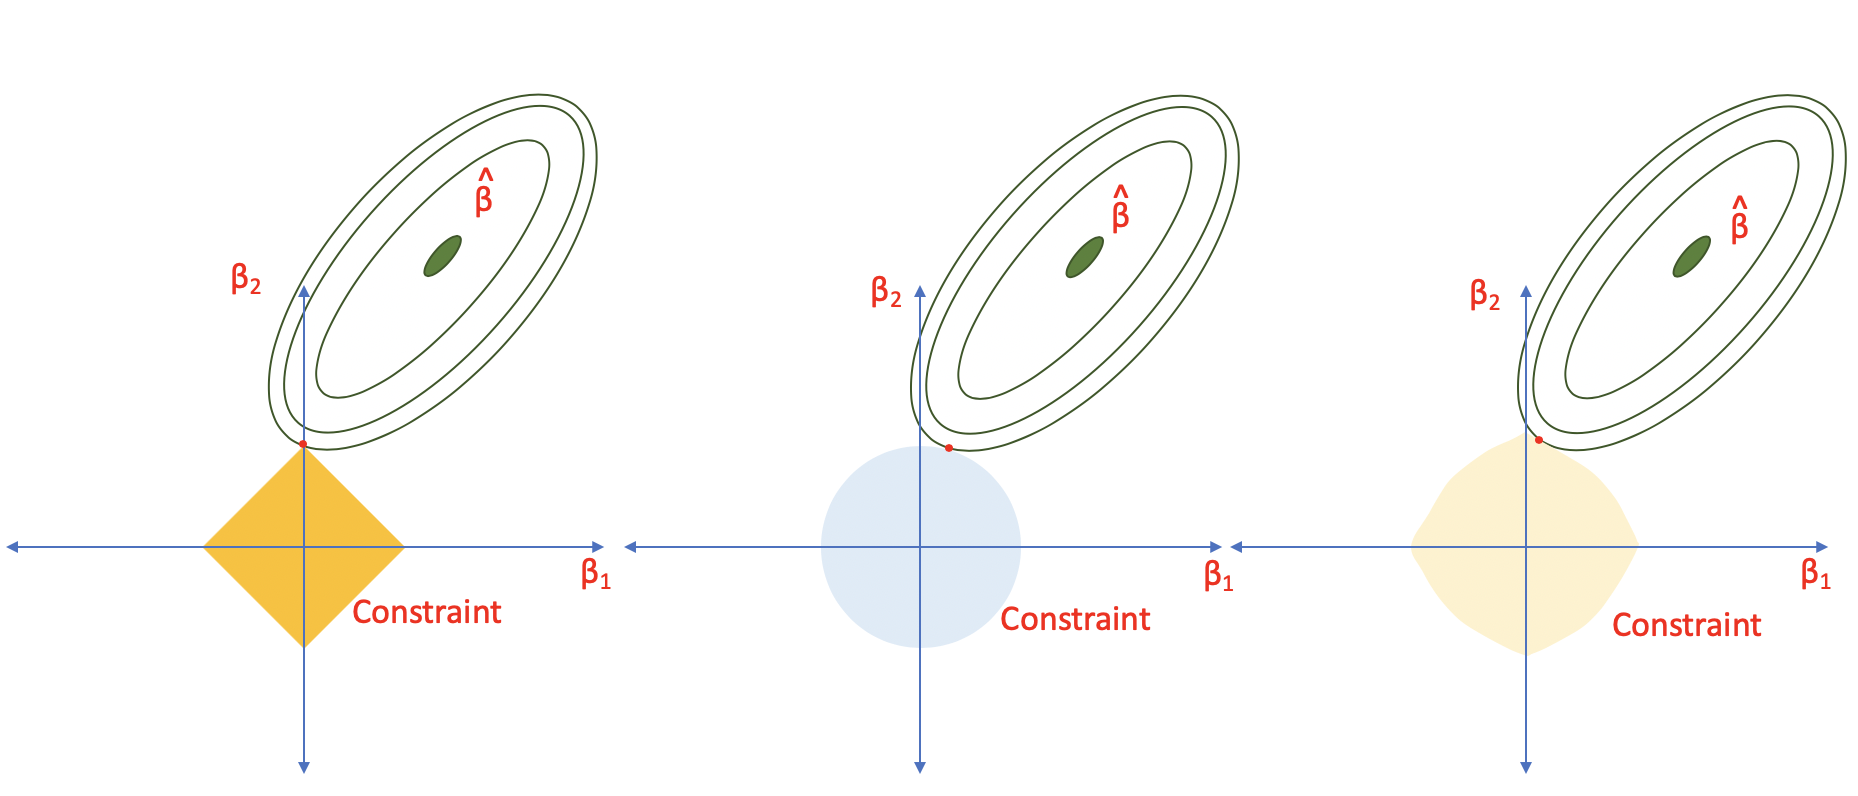
\includegraphics[width = 150mm, scale = 0.75]{penalised models graphs}
\end{center}

So what can be seen here from the three penalisation model graphs are three differing shapes for the constraint regions. The ellipses represent the contours of the RSS values away from the OLS. The constraint regions will increase in size as \(\lambda \to 0\) which would bring the \(\beta\) values to their OLS values. However, if  \(\lambda\)  does not equal zero then the constraint shrinks along with the \(\beta\) values as they are evaluated at the point where the RSS + penalty contours intersect with the constraint region. The reason why LASSO pushes some coefficients to zero is shown in these plots. Because of its diamond shape there is a possibility that the contours intersect with the constraint region on the axes. This is not possible with ridge regression since in OLS no coefficients have zero values and therefore the contours will not intersect the circular shape at the axes. The third plot from the right shows the constraint region for an elastic net which is the middle ground between LASSO and ridge regression. Here the coefficients may get pushed quite close to zero but will never reach it.

The plots show only a relationship between a dependent variable and two independent variables, hence the ability to plot this on an x-y plane. For more than two independent variables the plots get more complex and include further dimensions so they are very tricky to display on paper

\subsubsection{Random Forest}
To explain the random forest method, the concept of a decision tree must be established first\cite{Ibrahim2023}. At the beginning of constructing a decision tree \(100\%\) of the data constitutes what is labelled the root node\cite{SinghKushwah2022}. From there this node is split in two and then two again and so on. How these splits are determined is based on attributes of the independent variables used in the model. When training a decision tree the independent variables are used to determine how to split the data into the two new nodes, or leaves. Should a leaf be split in a way that minimises the mean squared error by a significant it will carry on splitting. Given this standard, a leaf that will not be split further is labelled a terminal node. Each terminal node includes a subset of the overall population of the dataset, and each individual is assigned a prediction of the dependent variable which is equivalent to the mean of the dependent variable values in the training set\cite{SpringerSeries}. Therefore when evaluating the model the test data would be fed into the tree and the predictions obtained depend on which leaf each individual falls into. The evaluation metric can then be calculated using these predictions and the actual values.

How the algorithm splits the data is determined by how much a variable or multiple variables minimise the mean squared error after the split\cite{Kitchin2020} and the same is true for the decision on which leaf to split further. In CART trees, classification and regression trees, only one variable is selected\cite{Ishwaran2015} and these are the type of trees that are used as the makeup for the ensemble random forest model. All univariate decision trees, by nature, follow the CART model in that only one variable is used to determine each split. However there are other multivariable models that use a linear composition of the variables to consider to determine the splits \cite{Yildiz2012}, tree algorithms such as oblique decision trees separate data in this way \cite{Wickramarachchi2015}, but these are not used in the random forest R function used in this report. 

As an example consider a univariate model where the price of a product, in a non-specific currency, is used to predict how many products are sold. The data consists of \(100\) products each of different prices and the total sales of each. The trained decision tree for this data is plotted as follows.

%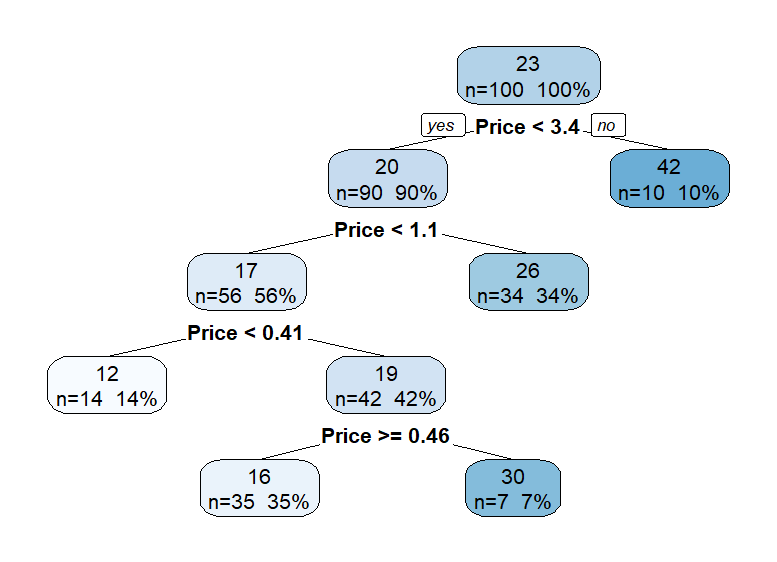
\includegraphics{example decision tree 2}
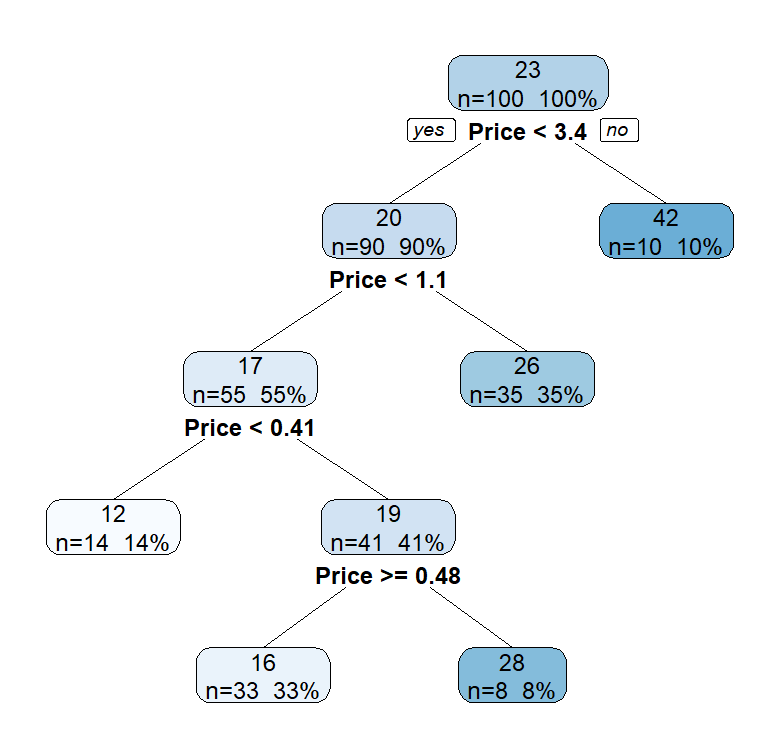
\includegraphics{decisiontree}

%Here if the price of the product is \(> 3.40\) the prediction for the amount sold is \(42\). The sales are predicted to be \(26\) for products sold between \(1.10\) and \(3.40\), products sold for less than \(0.41\)  have a predicted amount of \(12\),  for products sold between \(0,46\) and \(1.10\) have a predicted amount of 16 and finally the products sold with a price ranging from \(0.41\) and  \(0.46\) has a prediction of 30. Mostly this tree makes sense to show a coherent relationship between price of a product to the amount sold, however the figure of the predicted sales for the products priced between \(0.41\)and \(0.46\) doesn't follow the pattern. This is likely due to the fact that there is a small sample size in this section, \(n = 7\),  which may include some outliers that increase the mean average value. There are parameters that can be set to avoid this kind of issue. One is minsplit, which is the minimum number of individuals in the section for it to be split. This can help alleviate the final splits from having a small population and the predictions from being inaccurate. The depth of the tree can also be controlled with the maxdepth parameter.

From this figure you can see the cascading steps from node to node as the algorithm determines the prediction of the target variable. The value for which each split is decided upon is as described earlier, the algorithm will find the one split that has the most significant minimisation of the mean squared error. Since this example includes a relatively small sample population of data so there is bound to be some unusal predictions. Case in point the price values between 0.41 and 0.48 giving a sales prediction of 28, deviating strongly from the pattern of the association. This comes as a limitation of the single decision tree model, specifically one that has a small sample with some outliers, as it is prone to overfitting therefore not being so useful to predict unseen data.

%include graph of relationship
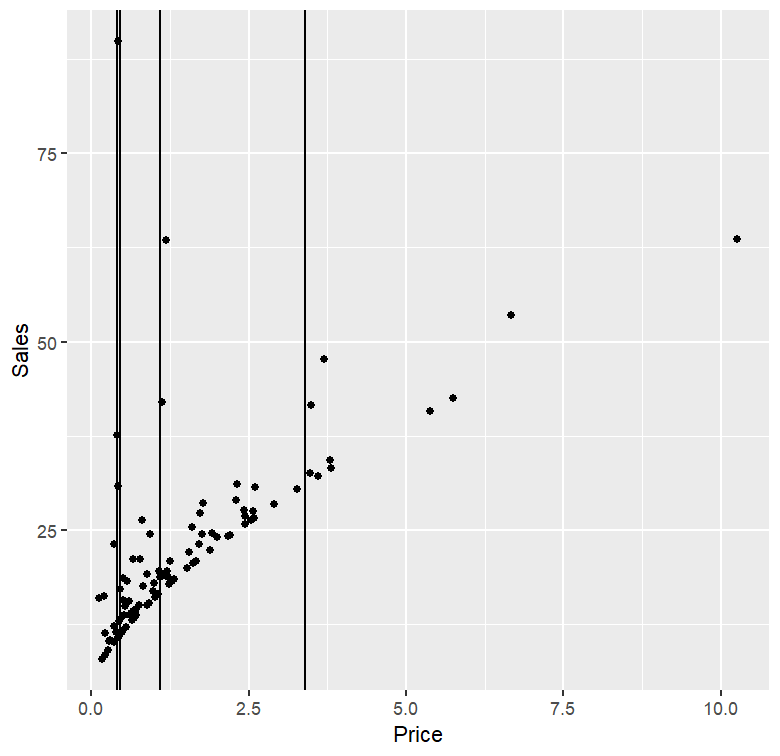
\includegraphics{decisionplot}

This is a graph visualisation of the data for the price of the product the products sales with lines that split the graph into sections according to the output of the decision tree model. Upon inspection it can be confirmed that the \(0.41 < 0.48\) price group does in fact include a very significant outlier and other higher values than would be expected for that section therefore resulting in an unusually increased prediction.

It is worth noting that this data has been randomly generated and in no way models the actual relationship between the price of a product and its subsequent sales figures.

This example and explanation of basic decision trees lays the groundwork for the explanation of random forest prediction models.

Random forest is an ensemble method, one that is an ensemble of multiple decision trees\cite{Biau2015}. This model applies a bootstrapping aggregation, bagging, technique to sample with replacement from the training dataset to create D new datasets that will be used to train D trees\cite{Breiman2001}, where the number of trees can be tuned as a parameter of the model. With random forest the number of variables randomly selected to consider for each split is limited by the hyperparameter mtry, a value that will always be less than the number of predictor variables. A larger mtry value will increase the amount of bias whereas the a low mtry value will increase the amount of variance, so finding the optimal value is key to find a middle ground in balancing the variance and the bias. This hyperparameter is very influential as it is what separates the random forest out from other ensemble decision tree models. The D trees therefore constitue the forest part of the algorithm each giving separate predictions for the data. The next step of the algorthim is to aggregate the predictions from each of the trees. Since this is done with a k-cross validation these steps are repeated k times. Then the model can be evaluated according to the process of using the test dataset to test the model and produce the values for the performance metrics. 

To tune the hyperparameters, such as number of trees and mtry, it is useful to visualise their effect on the variance as their value increases. Then it would be much easier to determine the optimal values of the parameters, those that allow for an effective model without introducing too much computational intensity.

 %to cp decides whether there should be another split, training dataset gets split into D bootstrapped datasets, only m predictors out of the p are selected to decide the trees different for each D dataset, determine the number of predictors to be considered at each split, determine number of trees, evaluate these hyperparameters with a graph which should show the values of the hyperparameters after which there is no significant decrease in the error - an excessively large hyperparameter will increase model complexity and computational intensiveness

\subsection{Evaluation of Prediction Models}
It is important to consider the validity of prediction models. There are several methods that are designed to check the generalisability of how well models fit to new data which can be assessed both using either internal or external validation\cite{Jiang2017}. A prediction model needs to go through this process of validation so that it can be compared with other models and also it assists in determining whether the model may be suitable for use in practice.

A common method of internal validation is k-fold cross-validation\cite{Rodrguez2013}. This involves splitting the dataset into k folds, usually k is set to 5 or 10, one split is used as the test dataset and the others used to train the model. In this way, all the data is used both to train and test. The performance metrics in each fold can be evaluated using the predictions and actual values for the test set. k-fold cross-validation is an improvement on the simpler method of split-sampling, which is essentially a cruder version of the method. Split-sampling could be thought of as equivalent to a 1-fold cross-validation just without rotation on different folds as the data is split into only one training set and one test set. The reduced use of the complete data to both train and test, as is the case in cross validation, introduces a higher level of variability and bias in estimating the performance of the model\cite{Varma2006}. This is why the cross validation technique is highly favoured in comparison.

Leave one out cross-validation is a special case of the k-fold cross-validation method. In this case if there are n records in the dataset then there would be n folds. Effectively in each iteration there is a training dataset of size n-1 and a test set of 1. How this method is performed and evaluated is identical to the k-fold, where k is n. The main advantage of this method over cross validation for a smaller k, is that since in each iteration the model is trained on almost the complete dataset, n-1, so there is a very low bias. Some significant disadvantages, however, is a high variance in the estimator, and a further instability due to outliers in the data or model sensitvity. This is stated quite succintly by Hastie et al, with "k = n, the cross-validation estimator is approximately unbiased for the true (expected) prediction error, but can have high variance because the n “training sets” are so similar to one another" \cite{SpringerSeries}. Quite often the computational cost disadvantage of running n iterations of training and evaluating the data, is enough to find the leave one out method as unsuitable. Datasets of size beyond ~1000 are typically not suited to this method because of this. So all things considered, the leave one out method is less useful in this specific study compared to standard cross-validation.

Bootstrap validation is a sophisticated technique that, since about the 1980s/1990s, has become a viable method of model validation for use on larger datasets due to increased computing power.  The bootstrapping method attempts to adjust for the optimism in the performance estimate therefore reducing its bias. Iba et al note that a multivariable prediction model's ""apparent" predictive performances such as discrimination and calibration calculation in the derivation dataset are better than the actual performance for an external population"\cite{Iba2021}. The optimism is then defined as the described difference between the performance on the "derivation dataset" and the performance for an external populaiton. The process involves creating M new datasets of size N from the original dataset. Each of the new datasets may include multiple of the same records found in the original as they are sampled with replacement \cite{Henderson2005}. The first iteration involves getting the performance from the original dataset and the performance for the bootstrapped dataset. The optimism of each model can be derived from these two performance values by subtracting the performance on the bootstrapped dataset from the performance on the full dataset. The optimism is averaged over the M bootstrapped datasets to give an average optimism value. Subtracting this value from the full dataset's performance estimation gives the value for optimism-adjusted performance estimation. This bias in the new performance estimation is reduced because the size of the dataset used to train the model is equivalent to the original dataset as opposed to the shrinking of the cross validation techniques.
Similar to leave one out cross-validation bootstrapping in comparison to k-fold cross-validation is better when the dataset is smaller due to the increased computational complexity and decreased effectiveness in larger datasets.

The validation method used in this study will be k-fold cross-validation due to its managable computational intensity and its ability to work well with larger datasets.

The best way to validate a machine learning prediction model is to validate externally. A model validated only on the data included in the original dataset still carries a lot of optimism and may fit poorly. Evaluation on relevant data obtained in new settings gives a better estimate of how generalisable the model is to a diverse range of populations. The more external validations performed with a more varied array of data provide a greater picture of the generalisability. This is important because if the model is applied to populations with demographics dissimilar to those represented in the training or testing data, the likelihood of inaccurate predictions increases. Inaccurate predictions lead to inefficiencies that reduce the model's usefulness.

\subsubsection{Nested Cross Validation}
A simple k-fold cross-validation is prone to some bias. A way to reduce this bias is to use a process of cross-validation within each fold, which is a method commonly known as nested cross-validation. A visualisation of the process is given in figure 8 of this paper\cite{Bates2022}, it shows how the train dataset is split for cross-validation. The bias that arises in standard cross-validation stems from the fact that the test data used in evaluation will also be used in hyperparameter tuning, essentially saying the test set has been peeked at in the process. The bias affects the accuracy of the performance evaluation, so it should be reduced as much as possible. The nested approach minimises the bias significantly by tuning the hyperparameters solely on the train datasets. These points echo the understanding that, Krstajic et al \cite{Krstajic2014}, present. Of course the downside of nested cross-validation is the increased rounds of training and testing which leads to a high level of computational complexity that may dissuade its usage depending on the computational power at hand.

\subsubsection{Cross Validation to Imputation Pipeline}
To evaluate the performance of the models it's important to consider the order of pre-processing (imputation) and cross validation. The order is important for reducing data leakage\cite{Dataleakage}, which introduces optimistically biased predictions of the observed data causing the reduction of the suitability for use of the model to make predictions on unseen data.

By imputing first, the data is imputed only once, so any data used in validation affects the way in which the missing data is imputed thereby leading to a significant amount of data leakage. In comparison by using an imputation within each cross validation fold approach the data leakage is nullified because the data from the test dataset never affects the imputation of the data used to train the model. So in terms of avoiding data leakage the order of imputation within the cross validation would be preferred; the evaluation that imputation within cross validation outputs is less optimistically bias and closer to the true evaluation to the model's ability to predict accurately on unseen data. 

Imputation before cross validation before cross validation results in a lower variability whereas imputation within cross validation results in a higher variability. In a validation process there a several sources that affect the level of variance. With the core structure of the two approaches in question the only source of variance that separates the two is how the imputation is applied. Imputing the whole dataset before it's split up into folds means that the variance gained from imputation is only appended to the total one time. In contrast, for the opposing approach, imputation is conducted within each fold and therefore the total variance will be higher in this scenario. A lower variability in the prediction model leads to more stable predictions as the confidence interval is low. In the case of ICU length of stay, a low variability would therfore predict stays of similar lengths with very little room for outliers. High variability introduces a greater amount of noise and is much more well accounted for picking up on outliers. This is beneficial for predicting the nature of ICU length of stay as there can be stays that last condsiderably longer than predicted unless high variability is accounted for. In some instances low variability would be the more suitable option but due to the data leakage and the context the order of imputation within cross validation with its high variability is favoured.

So with the decision made that the order of imputation within cross validation as the more suitable choice a visualisation is useful to properly show how this works.

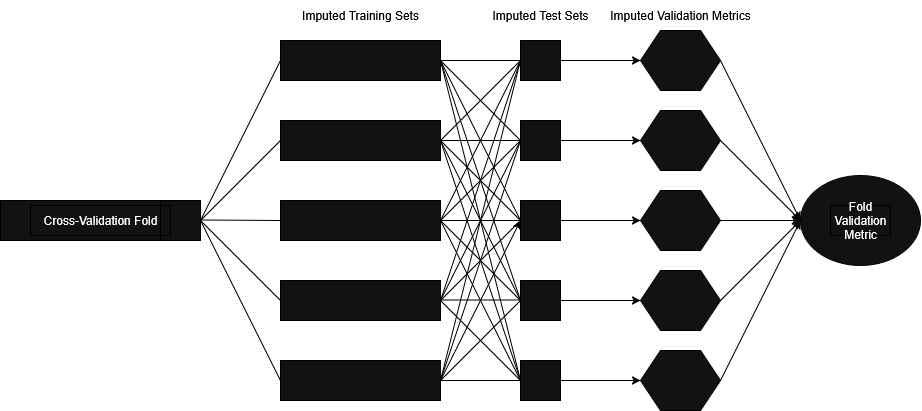
\includegraphics[width = 150mm, scale = 0.75]{imputedcv11}

This visualisation shows how to implement the MICE imputation process within one cross validation fold to produce a value of the validation metric. The cross validation fold with missing data is imputed five separate times. The train set is imputed first, then the corresponding test set is imputed by using the imputer devepoloped when imputing the train set. Since the order of the validation is imputation within cross validation each imputed set of train and test sets should be validated against each other. This is shown in the figure by the various arrows representing the many-to-many validation to produce five validation metrics values, these are averaged to obtain the value of the validation metric for this fold. This value is used amongst the other values of the fold validation folds to produce the final validation value of the final model.

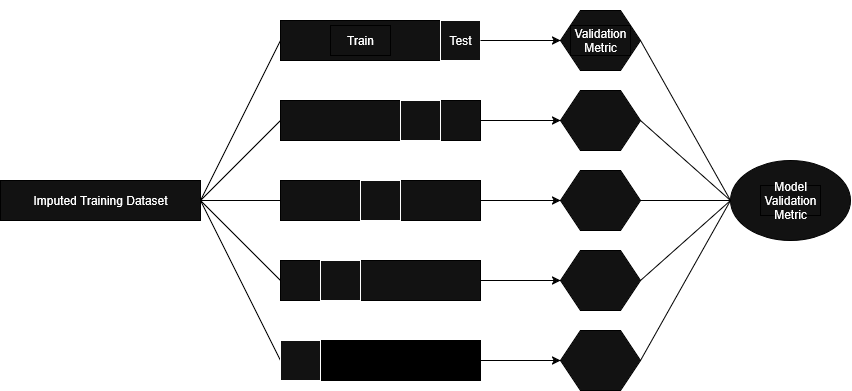
\includegraphics[width = 150mm, scale = 0.75]{cv7}

This figure visualises the inner loop of nested cross-validation which is the result of the decision to add a layer of cross validation within each fold. As shown, each imputed train dataset is taken and split into k-folds, just as in the outer loop. The process then plays out as a standard k-fold cross validation as is detailed above. This repeats in an iterative fashion as it cycles through values of the hyperparamer, which this inner loop attempts to tune.


%To properly assess the performance of a model that is trained with data that has missing values needs to go through both a cross validation and imputation step. It is important to consider the details of the process, mainly deciding the order of the application of the pre-processing imputation and the validation methods. The reason this is so important is due to the need to reduce data leakage in the model. This particular type of leakage is named test-to-train leakage and it describes the idea that if imputation is done before the dataset is split into k-folds there will be leakage because in the process of imputation the test data will be used to affect the imputed data in the training dataset, which is a problem because the test set should be unseen data that has no interference in the training set. So therefore to avoid this type of data leakage it would be advisable to impute the train and test set separately within each cross-validated fold.

%When training a given model the amount of seperate models created in this process is equivalent to \(K \cdot M\) where \(K\) is the number of folds used for cross-validation and \(M\) is the number of imputed datasets within each fold. The ultimate aim when training a machine learning model is to have only one model, so the \(K \cdot M \) models will have to be aggregated into one. talk about the with() function and what that does and then talk about the pool function and what that does, then about evaluating the aggregated test sets on the pooled model. The performance metrics will be averaged

%include diagram of the with and pool process to get the final model

%\subsection{Feature Importance}
%After obtaining each of the models it is useful to compare how much of an impact each of the variables has on the prediction of the dependent variable.

%\subsection{Data Augmentation}
%Data augmentation is the process of enhancing a dataset by applying transformations to the original data to generate additional data. It may be of interest to augment the data as there is a possibility that it could improve the model's accuracy and help it fit better to unseen data.

\section{Results}

\subsection{Dataset Description}

\subsubsection{Data Extraction}

The MIMIC-IV dataset provides data on 364,627 unique individuals who give 546,028 hospitalisations with 94,458 unique ICU stays. To identify the lung cancer ICU stays the data in the ICU stays table must be sifted through by the ICD-9 and ICD-10 codes that identify lung cancer. Data is removed if it is outside of the normal range in any of the variables. After doing this the number of ICU stays for patients with lung cancer comes to a value of 2,390, sourced from 2,115 unique admissions.

An admission may have multiple ICU stays recognised within the dataset. If two concurrent ICU stays are less than or equal to 24 hours apart their lengths of stay are added together and treated as one stay. If this is not the case they will be treated as two separate ICU stays. A column is created to differentiate the ICU stays from the same admission marking the number of previous stays. This reduction leaves the dataset with 2,303 ICU stays.

The flowchart in figure ... below shows how the ICU stays, used in the prediction models, are extracted from the MIMIC-IV dataset.

\subsubsection{ICU Stay Demographics}

Among the 2,303 ICU stays there is a slight favour of males, \(54\%\), to females, \(46\%\).  The most populous age range is the 61-70  year old group, \(33.4\%\), followed by the 71-80 group, \(29.0\%\). The 18-40 group is markedly small, \(0.6\%\),  given it's wide range. The majority of patients' ICU stays, included in this dataset, are of white ethnicity, \(72.6\%\), and the majority of patients are in hospital with medicare insurance , \(61.6\%\). Over half of the stays, \(55.5\%\) were from the result of emergency admissions. More detailed statistics is given in table 1.

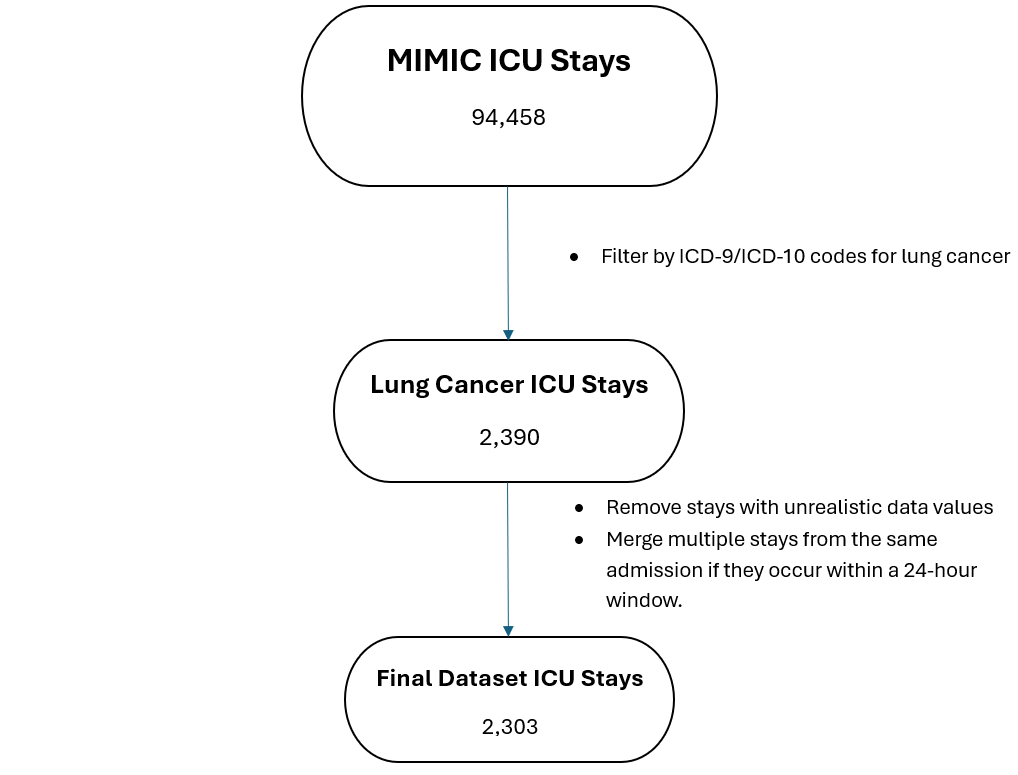
\includegraphics[width = 150mm, scale = 0.75]{flowchart}


{\seriffont
{\small
\renewcommand{\arraystretch}{1}
%\centering
\begin{center}

\setlength{\arrayrulewidth}{0.7mm}
\begin{longtable}{ |L{7.5cm} | L{6cm} |} 
    \hline
    \textbf{Characteristic} & \textbf{N = 2303}\\
    \noalign{\global\setlength{\arrayrulewidth}{0.7mm}}
    \hline
    \endfirsthead

    \hline 
    \textbf{Characteristic} & \textbf{N = 2303}\\
    \hline
    \endhead
    \multicolumn{2}{|p{13.5cm}|}{\textbf{Number of previous ICU stays (within hospital admission)}} \\
    \hline
        0  & 2,115 (92.0\%) \\ 
    \noalign{\global\setlength{\arrayrulewidth}{0.05mm}}
    \hline
    \noalign{\global\setlength{\arrayrulewidth}{0.7mm}}
        1  & 171 (7.4\%) \\
    \noalign{\global\setlength{\arrayrulewidth}{0.05mm}}
    \hline
    \noalign{\global\setlength{\arrayrulewidth}{0.7mm}}
        2  & 13 (0.6\%) \\
    \noalign{\global\setlength{\arrayrulewidth}{0.05mm}}
    \hline
    \noalign{\global\setlength{\arrayrulewidth}{0.7mm}}
        3 & 3 (0.1\%) \\
    \noalign{\global\setlength{\arrayrulewidth}{0.05mm}}
    \hline
    \noalign{\global\setlength{\arrayrulewidth}{0.7mm}}
        4 & 1 (<0.1\%) \\
    \hline
    \multicolumn{2}{|p{13.5cm}|}{\textbf{Age (years)}} \\
    \hline
       18-40   & 14 (0.6\%)\\
    \noalign{\global\setlength{\arrayrulewidth}{0.05mm}}
    \hline
    \noalign{\global\setlength{\arrayrulewidth}{0.7mm}}
       41-50   & 93 (4.0\%)\\
    \noalign{\global\setlength{\arrayrulewidth}{0.05mm}}
    \hline
    \noalign{\global\setlength{\arrayrulewidth}{0.7mm}}
       51-60   & 386 (16.8\%)\\
    \noalign{\global\setlength{\arrayrulewidth}{0.05mm}}
    \hline
    \noalign{\global\setlength{\arrayrulewidth}{0.7mm}}
       61-70   & 769 (33.4\%)\\
    \noalign{\global\setlength{\arrayrulewidth}{0.05mm}}
    \hline
    \noalign{\global\setlength{\arrayrulewidth}{0.7mm}}
       71-80   & 668 (29.0\%)\\
    \noalign{\global\setlength{\arrayrulewidth}{0.05mm}}
    \hline
    \noalign{\global\setlength{\arrayrulewidth}{0.7mm}}
       81-90   & 318 (13.8\%)\\
    \noalign{\global\setlength{\arrayrulewidth}{0.05mm}}
    \hline
    \noalign{\global\setlength{\arrayrulewidth}{0.7mm}}
       91+     & 55 (2.4\%)\\
    \hline
    \multicolumn{2}{|p{13.5cm}|}{\textbf{Sex}} \\
    \hline
       Male  & 1,237 (54\%) \\
    \noalign{\global\setlength{\arrayrulewidth}{0.05mm}}
    \hline
    \noalign{\global\setlength{\arrayrulewidth}{0.7mm}}
       Female  & 1,066 (46\%) \\
    \hline
    \multicolumn{2}{|p{13.5cm}|}{\textbf{Ethnicity}} \\
    \hline
       White  & 1,671 (72.6\%) \\
    \noalign{\global\setlength{\arrayrulewidth}{0.05mm}}
    \hline
    \noalign{\global\setlength{\arrayrulewidth}{0.7mm}}
       Black  & 217 (9.4\%) \\
    \noalign{\global\setlength{\arrayrulewidth}{0.05mm}}
    \hline
    \noalign{\global\setlength{\arrayrulewidth}{0.7mm}}
       Asian  & 122 (5.3\%) \\
    \noalign{\global\setlength{\arrayrulewidth}{0.05mm}}
    \hline
    \noalign{\global\setlength{\arrayrulewidth}{0.7mm}}
       Hispanic/Latino  & 49 (2.1\%) \\
    \noalign{\global\setlength{\arrayrulewidth}{0.05mm}}
    \hline
    \noalign{\global\setlength{\arrayrulewidth}{0.7mm}}
       Other & 66 (2.9\%) \\
    \noalign{\global\setlength{\arrayrulewidth}{0.05mm}}
    \hline
    \noalign{\global\setlength{\arrayrulewidth}{0.7mm}}
       Missing & 178 (7.7\%) \\
    \hline
    \multicolumn{2}{|p{13.5cm}|}{\textbf{Insurance}} \\
    \hline
       Medicare  & 1,418 (61.6\%) \\
    \noalign{\global\setlength{\arrayrulewidth}{0.05mm}}
    \hline
    \noalign{\global\setlength{\arrayrulewidth}{0.7mm}}
       Private   & 537 (23.3\%) \\
    \noalign{\global\setlength{\arrayrulewidth}{0.05mm}}
    \hline
    \noalign{\global\setlength{\arrayrulewidth}{0.7mm}}
       Medicaid  & 288 (12.5\%) \\
    \noalign{\global\setlength{\arrayrulewidth}{0.05mm}}
    \hline
    \noalign{\global\setlength{\arrayrulewidth}{0.7mm}}
       Other  & 44 (1.9\%) \\
    \noalign{\global\setlength{\arrayrulewidth}{0.05mm}}
    \hline
    \noalign{\global\setlength{\arrayrulewidth}{0.7mm}}
       Missing  & 16 (0.7\%) \\
    \hline
    \multicolumn{2}{|p{13.5cm}|}{\textbf{Admission Type}} \\
    \hline
       Emergency & 1,278 (55.5\%) \\
    \noalign{\global\setlength{\arrayrulewidth}{0.05mm}}
    \hline
    \noalign{\global\setlength{\arrayrulewidth}{0.7mm}}
       Observation & 365 (15.9\%) \\
    \noalign{\global\setlength{\arrayrulewidth}{0.05mm}}
    \hline
    \noalign{\global\setlength{\arrayrulewidth}{0.7mm}}
       Urgent & 335 (14.5\%) \\
    \noalign{\global\setlength{\arrayrulewidth}{0.05mm}}
    \hline
    \noalign{\global\setlength{\arrayrulewidth}{0.7mm}}
       Elective & 325 (14.1\%) \\
    \hline
    \multicolumn{2}{|p{13.5cm}|}{\textbf{Platelets (k/µL)}} \\
    \hline
       Mean (SD) & 265.8 (133.1) \\
    \noalign{\global\setlength{\arrayrulewidth}{0.05mm}}
    \hline
    \noalign{\global\setlength{\arrayrulewidth}{0.7mm}}
       N missing (\%) & 1,347 (58.5) \\
    \hline
    \multicolumn{2}{|p{13.5cm}|}{\textbf{Glucose (mg/dL)}} \\
    \hline
       Mean (SD) & 137.2 (78.9) \\
    \noalign{\global\setlength{\arrayrulewidth}{0.05mm}}
    \hline
    \noalign{\global\setlength{\arrayrulewidth}{0.7mm}}
       N missing (\%) & 1,252 (54.4) \\
    \hline
    \multicolumn{2}{|p{13.5cm}|}{\textbf{Chloride (mEq/L)}} \\
    \hline
       Mean (SD) & 100.4 (8.0) \\
    \noalign{\global\setlength{\arrayrulewidth}{0.05mm}}
    \hline
    \noalign{\global\setlength{\arrayrulewidth}{0.7mm}}
       N missing (\%) & 1,259 (54.7) \\
    \hline
    \multicolumn{2}{|p{13.5cm}|}{\textbf{Potassium (mEq/L)}} \\
    \hline
       Mean (SD) & 4.7 (4.9)\\
    \noalign{\global\setlength{\arrayrulewidth}{0.05mm}}
    \hline
    \noalign{\global\setlength{\arrayrulewidth}{0.7mm}}
       N missing & 1,244 (54.0)\\
    \hline
    \multicolumn{2}{|p{13.5cm}|}{\textbf{Haemoglobin (g/dL)}} \\
    \hline
       Mean (SD) & 10.6 (2.6) \\
    \noalign{\global\setlength{\arrayrulewidth}{0.05mm}}
    \hline
    \noalign{\global\setlength{\arrayrulewidth}{0.7mm}}
       N missing (\%) & 1,258 (54.6) \\
    \hline
    \multicolumn{2}{|p{13.5cm}|}{\textbf{Haematocrit (\%)}} \\
    \hline
       Mean (SD) & 32.7 (6.7) \\
    \noalign{\global\setlength{\arrayrulewidth}{0.05mm}}
    \hline
    \noalign{\global\setlength{\arrayrulewidth}{0.7mm}}
       N missing (\%) & 1,249 (54.2) \\
    \hline
    \multicolumn{2}{|p{13.5cm}|}{\textbf{Sodium (mEq/L)}} \\
    \hline
       Mean (SD) & 135.3 (13.0) \\
    \noalign{\global\setlength{\arrayrulewidth}{0.05mm}}
    \hline
    \noalign{\global\setlength{\arrayrulewidth}{0.7mm}}
       N missing (\%) & 1,250 (54.3) \\
    \hline
    \multicolumn{2}{|p{13.5cm}|}{\textbf{Drugs taken}} \\
    \hline
       Ondansetron & 397 (17.2\%) \\
    \noalign{\global\setlength{\arrayrulewidth}{0.05mm}}
    \hline
    \noalign{\global\setlength{\arrayrulewidth}{0.7mm}}
       Calcium Gluconate & 926 (40.2\%) \\
    \hline
    \multicolumn{2}{|p{13.5cm}|}{\textbf{Death in ICU}} \\
    \hline
       Survived & 1775 (77.1\%) \\
    \noalign{\global\setlength{\arrayrulewidth}{0.05mm}}
    \hline
    \noalign{\global\setlength{\arrayrulewidth}{0.7mm}}
       Deceased & 528 (22.9\%) \\
    \hline
    \multicolumn{2}{|p{13.5cm}|}{\textbf{Length of stay (days)}} \\
    \hline
       Mean (SD) & 3.9 (5.2) \\
    \hline
    \caption{Caption}
    \label{tab:my_label}
\end{longtable}
\end{center}}
\normalsize

\subsection{Missing Data}


\includegraphics[width = 150mm, scale = 0.75]{missing_data}

All of the data variables shown in this graph have highly significant amounts of missing data with not one variable showing a percentage of missing data less than 50 \%\.  This is not very conducive for the inclusion of these variables in the prediction models since when data is more than 40 \%\ missing it can only be considered as hypothesis generating and therefore will likely not provide accurate predictions. However, some data must be used so for the purposes of the continuation of the study the variables in green are kept as predictors in the model. 

\subsection{Imputation}

\subsubsection{Correlation Plot}

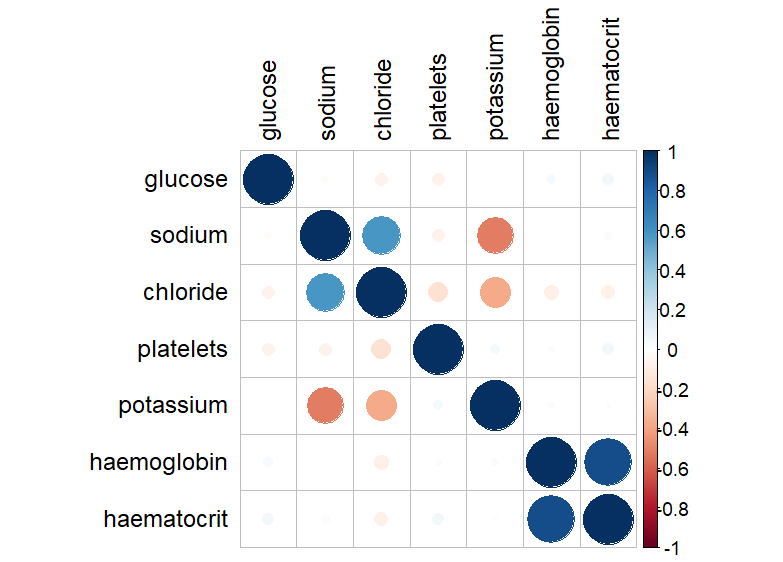
\includegraphics[width = 150mm, scale = 0.75]{correlation}

The correlation graph shows that most of the variables are not significantly correlated enough that it would affect the imputation process by not enabling the model to converge for all variables. However the haematocrit and the haemoglobin variables are very significantly correlated, and therefore they have high levels of multicolinearity, which should hinder the models potential to converge and produce reliable imputed data. An adjustment to the prediction matrix is needed to remove the relationship between haematocrit and haemoglobin from the imputation process.

\subsubsection{Trace Plots}

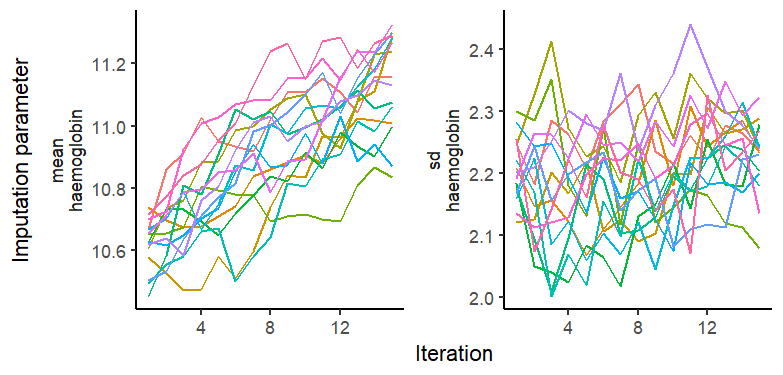
\includegraphics[width = 150mm, scale = 0.75]{trace_haemo1}

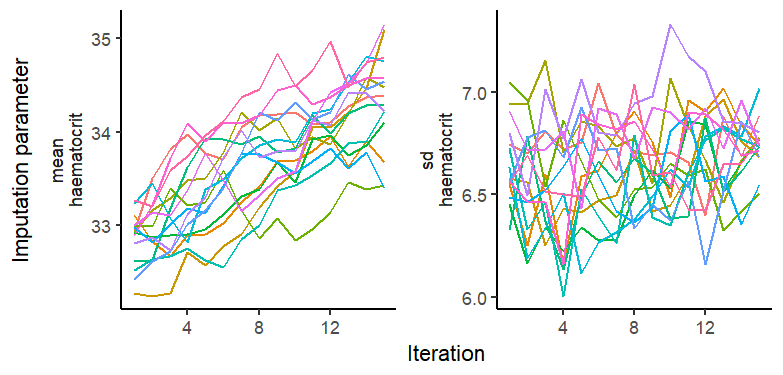
\includegraphics[width = 150mm, scale = 0.75]{trace_haema1}

Clearly shown in the trace plots above the mean of the data for both the haemoglobin and the haematocrit variables tends to increase with each imputation iteration. Ideally there should be a point where the mean should remain mostly unchangable from iteration to iteration. To fix this the predictor matrix should be amended. The way to do this is to not have the haematocrit be influential on the imputation of the haemoglobin and vice versa. The predictor matrix determines this with the use of binary inputs. The default is a matrix full of 1s which allows for an imputation where every variable affects the imputation of each other. By changing the 1s that refer to the haematocrit/haemoglobin interaction to 0 the trace plots should be corrected.

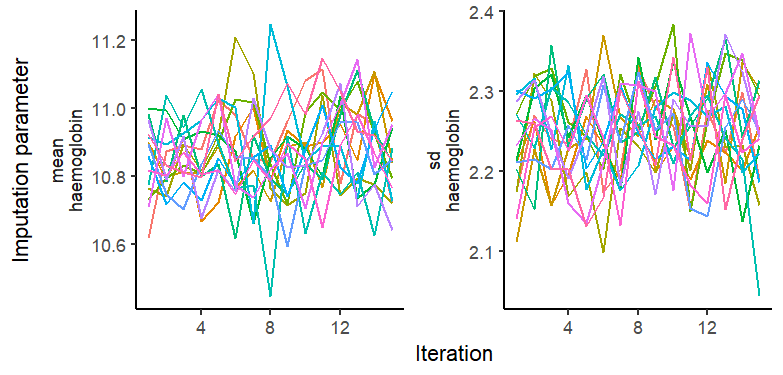
\includegraphics[width = 150mm, scale = 0.75]{trace_haemo2}

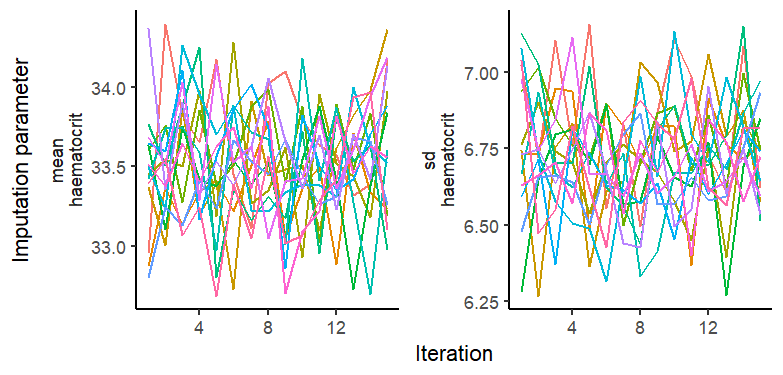
\includegraphics[width = 150mm, scale = 0.75]{trace_haema2}

These plots show a more correct imputation where the mean reaches a point where it remains mostly unchangable from iteration to iteration.

\subsubsection{Categorical Missing Values}

%\subsection{Prediction Models}

%\subsubsection{Linear Regression}

%\subsubsection{Penalisation Models}

%\subsubsection{Random Forest}

\subsection{Model Performance}

%\subsection{Variable Importance}


\section{Discussion}

\section{Conclusion}

\printbibliography

\section*{Appendix}
\addcontentsline{toc}{section}{Appendices}

\end{document}

